\chapter{Segmentación y Alineación automática}

Como la creación de recursos de manera manual es costosa, y los requerimientos de volúmen de información son altos, la generación automática o semi automática de recursos de habla toma gran relevancia en la investigación actual.

El procesamiento de grabaciones del dominio público para la creación de recursos para la investigación requiere la resolución de dos tareas concretas, que son la segmentación y la anotación definidas en el capítulo anterior.

\section{Segmentación basada en silencio}

Las segmentación basada en silencio es una respuesta natural al problema de como segmentar señales de voz, pues existe una correspondencia directa entre símbolos de puntuación y pausas en la voz. De igual manera en una señal de voz, los locutores requieren pausas para tomar aire, lo que permite que exista una cadencia en la señal y espacios donde realizar los cortes.

Para identificar el proceso de segmentación por silencios, es necesario entender cómo se almacenan las señales de voz digitalmente y cómo se puede procesar este tipo de datos.

La manera mas sencilla de representar digitalmente una señal de voz es haciendo el uso de la Modulación por Impulsos Codificados o PCM por sus siglas en inglés, donde por medio de un transductor análogo, se capturan las variaciones en la presión del aire y se registran como un rango de valores normalizado. El senso de la señal se hace periódicamente a una frecuencia determinada generando de esta manera una secuencia de valores que representa la señal. El proceso de representar la presión del aire en un segmento de tiempo se denomina cuantización, y para señales de audio se utilizan valores normalizados entre -127 y 128 representados por 8 bits a 16000 Hz de frecuencia.

En al figura \ref{img:pcm} se muestra la visualización de una grabación correspondiente a la palabra agua, extraída del corpus Open Speech Corpus de palabaras, en su longitud original y aumentada en un 500\% y 1000\% usando Audacity \cite{audacity}

\begin{figure}[H]
\caption{Representación visual de una señal de voz}
\label{img:pcm}
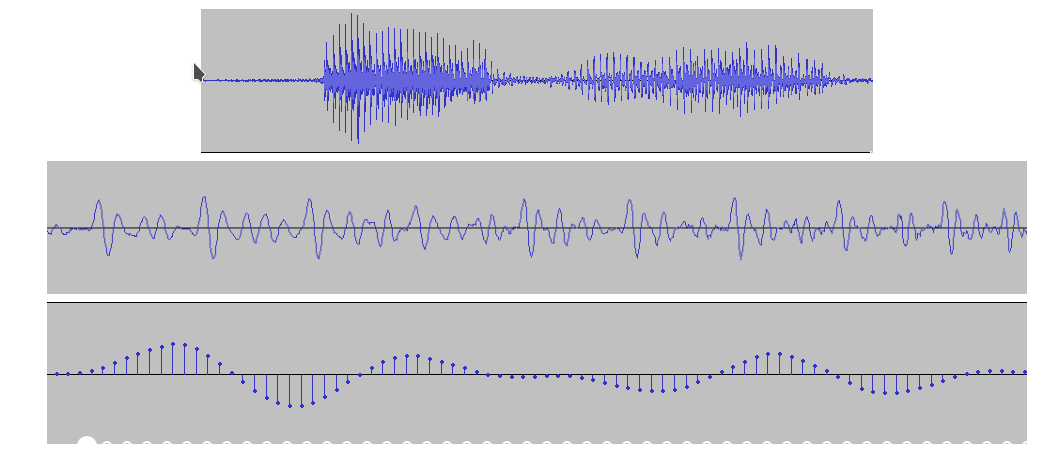
\includegraphics[width=\textwidth]{imagenes/04_01_pcm.png}
\end{figure}

Al hablar de silencio, nos referimos a ausencia total o parcial de sonido, lo cual se puede relacionar directamente con la intensidad de la señal en un segmento de tiempo.

Definiremos intensidad como la sumatoria de las energías en un periodo de tiempo  \cite{Jurafsky2000SpeechRecognition}    

\begin{equation}
\label{eq:energy}
I = \sum{x^2}  
\end{equation}

Esto nos daría un indicador de toda la señal, sin embargo, es útil realizar este análisis por pequeños segmentos del audio para identificar en conjunto cuales son los puntos donde la intensidad baja representa un espacio de silencio. Estos segmentos por lo general se definen en espacios de 25ms solapados cada 10ms \cite{Jurafsky2000SpeechRecognition}, lo cual da la idea de una señal continua, donde cada segmento comparte información con el anterior. 

Utilizando esta idea es posible tomar cualquier señal de voz, segmentarla cada 25ms y encontrar los segmentos consecutivos donde la intensidad sea baja o cercana a cero y estos segmentos consecutivos representarían pausas de silencio. Algunas consideraciones a tomar al usar esta aproximación es que incluso en medio de las señales de voz, existen subsegmentos donde la intensidad es baja, por ejemplo en la pronunciación de consonantes plosivas, como la b, c, d, g, p y t existe una interrupción momentánea y completa del flujo de aire, causando momentáneamente segmentos de silencio.

Con base en las anotaciones del corpus de experimentación fonética se determinó que la duración promedio de cada consonante plosiva es inferior a los 100ms. También, extrayendo información del corpus de pruebas se determinó que los espacios de silencio son de aproximadamente 500ms. Con esta información se decidió utilizar segmentos 250ms de longitud y desplazamiento de 100ms. Se determinan como silencios los conjuntos de cinco o más segmentos consecutivos de intensidad baja.

El criterio de silencio seleccionado como baja intensidad de múltiples segmentos consecutivos plantea retos con respecto al valor concreto de energía para determinar silencio o señal. Considerando que los locutores no grabaron a un volúmen estándar y que la relación ruido señal varía en todas las grabaciones es distinta, se propusieron dos aproximaciones para determinar los segmentos de silencio, la primera normalizando los valores de la señal y definiendo un umbral fijo de intensidad en proporción al valor mas alto de la grabación, considerando valores de 0.3, 0.15 y 0.15 que representan umbrales de intensidad del 30\%, 15\%, y 5\%. También se experimentó utilizando algoritmos de agrupamiento con dos centroides iniciales en 0 y la intensidad máxima. Los resultados se presentan en la tabla \ref{tab:resultados_segmentacion_silencios}.

\begin{table}[H]
\centering
\caption{Resultados de la segmentación por silencios}
% \caption{Speech English Corpus}
\label{tab:resultados_segmentacion_silencios}
\begin{tabular}{|l|l|}
\hline
\textbf{Umbral} & \textbf{Precisión}  \\ \hline
Fijo 30\%       & 57.01\%             \\  \hline
Fija 15\%       & 83.26\%             \\  \hline
Fija 5\%        & 69.05\%             \\  \hline
Dinámico        & 74.53\%             \\  \hline
\end{tabular}
\end{table}


\section{Alineación basada en duración de fonemas}

La alineación consiste en, después de tener una segmentación por silencios en las grabaciones y una segmentación por símbolos de puntuación en la transcripción, encontrar la relación que existe entre los segmentos de audio y los de tokens del texto.

La primera aproximación ingenua que consiste en relacionar en orden los segmentos de voz y texto. El problema con esta aproximación consisten en que las pausas no necesariamente corresponden siempre a un símbolo de puntuación, pues en caso de oraciones largas, el locutor debe respirar, y en oraciones muy cortas, el locutor omite la pausa para dar continuidad a la lectura.

Resaltando que existe igualmente un orden secuencial entre ambos segmentos, la aproximación basada en la duración de fonemas utiliza la duración promedio de fonemas extraída del corpus fonético de experimentación y reportada en la tabla \ref{tab:duracion_promedio_fonemas}. Con esta información y transformando las letras de cada token a su correspondiente fonema, se obtiene una duración estimada de cada token, la cual puede ser usada para alinear con mayor precisión.


\begin{table}[H]
\centering
\caption{Distribución fonética}
\label{tab:duracion_promedio_fonemas}
\begin{tabular}{|l|l|l|}
\textbf{Fonema} &\multicolumn{1}{|p{2cm}|}{\textbf{Duración promedio}} & \multicolumn{1}{|p{2cm}|}{\textbf{Desviación estándar}} \\ \hline
sil & 0.6619 & 0.3700 \\ \hline
a   & 0.1421 & 0.0566 \\ \hline
o   & 0.1487 & 0.0607 \\ \hline
e   & 0.1204 & 0.0416 \\ \hline
n   & 0.1090 & 0.0442 \\ \hline
i   & 0.1294 & 0.0404 \\ \hline
l   & 0.1125 & 0.0530 \\ \hline
s   & 0.1811 & 0.1059 \\ \hline
t   & 0.0784 & 0.0507 \\ \hline
d   & 0.0877 & 0.0536 \\ \hline
R   & 0.0999 & 0.0517 \\ \hline
b   & 0.0826 & 0.0610 \\ \hline
r   & 0.0750 & 0.0254 \\ \hline
p   & 0.0692 & 0.0649 \\ \hline
j   & 0.1038 & 0.0659 \\ \hline
u   & 0.1441 & 0.0507 \\ \hline
m   & 0.1183 & 0.0515 \\ \hline
k   & 0.1224 & 0.0904 \\ \hline
g   & 0.1016 & 0.0970 \\ \hline
f   & 0.1402 & 0.0569  \\ \hline
c   & 0.1032 & 0.0838  \\ \hline
y   & 0.1118 & 0.0044  \\ \hline
C   & 0.1274 & 0.0248  \\ \hline
N   & 0.0575 & 0  \\ \hline
S   & 0.0927 & 0  \\ \hline
\end{tabular}
\end{table}

Este problema entonces se simplifica a uno de optimización donde dados dos arreglos numéricos, donde el primero representa la duración en segundos de cada segmento y el segundo la duración estimada de cada token, se debe encontrar una relación entre los índices de cada arreglo que minimice la diferencia de segundos entre los segmentos correspondientes.

\section{Segmentación basada en información acústica}

Las grabaciones voz no son señales estacionarias, pero al segmentar en pequeños trozos de tamaño inferior al de la duración de los fonemas, estos segmentos cuando pertenecen a vocales y consonantes sonoras son estacionarios.

Si bien las características morfológicas de los locutores modifican su timbre y tono de voz, a nivel acústico, la dicción de cada fonema es similar. En las vocales, que son los fonemas con más energía, las partes de la anatomía responsables de diferenciar los sonidos son la apertura de la glotis y la apertura de la boca. Lo cual da la idea que una descomposición acústica podría identificar este fenómeno.

Al descomponer cualquier señal utilizando la transformada de Fourier (ver equación \ref{eq:fourier}), se obtienen señales raíz de cada onda compleja. Con las señales de voz, los coeficientes máximos  en el orden ascendente de la frecuencia se denominan formantes, y el formante 1 (f1) y el formante 2 (f2) representan efectivamente el fenómeno efectuado por las cuerda vocales vibrando y la resonancia dad por la cavidad bucal. Los formantes son harmónicos, la captura de estos se da en señales de cualquier tipo, sea de voz u otro fenómeno acústico, como las señales generadas por instrumentos musicales. Todos los formantes F1,F2,F3, etc. corresponden al pulso excitativo de la glotis y la resonancia en el tracto vocal

\begin{equation}
\label{eq:fourier}    
f(x) = \frac{1}{2} \, a_{0} + \sum_{n=1}^{\infty} \left[
   a_{n}\,\mathbf{cos} (n\,x) + b_{n} \,\mathbf{sin} (n\,x) \right]
\end{equation}

Los formantes teóricos para las cinco vocales del español se muestran en la tabla \ref{tab:formantes_teoricos} tomada de \cite{Bradlow1995}. Dichos formantes fueron calculados promediando la medición de formantes F1 y F2 de varios locutores con dialecto peninsular.

\begin{table}[H]
\centering
\caption{Formantes teóricos para vocales del español.}
\label{tab:formantes_teoricos}
\begin{tabular}{|l|l|l|l|l|}
\hline
\textbf{Vocal} & \textbf{f1} & \textbf{f2} & \textbf{std f1} & \textbf{std f2} \\ \hline
a   & 638 & 36 & 1353 & 84 \\ \hline
e   & 458 & 42 & 1800 & 131 \\ \hline
i   & 286 & 6  & 2200 & 131 \\ \hline
o   & 460 & 19 & 1019 & 99 \\ \hline
u   & 300 & 20 & 992  & 121 \\ \hline

\end{tabular}
\end{table}

También se realizó una observación de las vocales calculando sus formantes basados en la información extra\macb{\'i}da de las palabras anotadas fonéticamente. Esta información se encuentra en la tabla \ref{tab:formantes_observador}. Los formantes fueron calculados con Parselmouth \cite{parselmouth}.

\begin{table}[H]
\centering
\caption{Formantes teóricos para vocales del español}
\label{tab:formantes_observador}
\begin{tabular}{|l|l|l|l|l|}
\hline
\textbf{Vocal} & \textbf{f1} & \textbf{f2} & \textbf{std f1} & \textbf{std f2} \\ \hline
a   & 682.84 & 1347.66 & 73.77 & 93.04 \\ \hline
e   & 494.84 & 1619.97 & 55.49 & 132.84\\ \hline
i   & 382.33 & 1657.33 & 50.65 & 155.24 \\ \hline
o   & 506.24 & 1101.14 & 60.20 & 170.64\\ \hline
u   & 434.77 & 984.185 & 50.32 & 193.66\\ \hline

\end{tabular}
\end{table}

A partir de esta información se realizaron experimentos buscando la precisión en la identificación de las vocales. Para ello se tomó la norma L1 de los dos primeros formantes, definiendo rango de aceptación, entre los 50Hz y 500Hz; y utilizando la desviación estándar de cada vocal como rango de aceptación. Adicionalmente a esto, se entrenó un algoritmo de agrupación no supervizado, K-means, inicializando los centroides en los formantes observados en el corpus de experimentación fonética. Los resultados se reportan en la tabla \ref{tab:resultados_vocales}

\input{tablas/04_05_segmentación_vocalica}

Para entender los bajos resultados presentados por la aproximación basada en los formantes observados y su desviación (55.73\% de precisión), se realizó un análisis visual sobre grabaciones con las vocales que se extrajeron del Open Speech Corpus. Se graficó simultaneamente la onda, los formantes F1 y F2 donde la intensidad superaba los 60 decibeles, es decir, $I > 60 dB$, y los formantes F1 y F2 promedio y sus desviaciones observados en el corpus. Las figuras \ref{img:formantes_a} y \ref{img:formantes_e}  muestran un ejemplo de dicho análisis. Los puntos indican los formantes calculados, en rojo F2 y en azúl F1, en verde la señal, en amarillo la intensidad y en rojo los valores observados para los formantes esperados y su desvuación.

% (Y explicar las lineas rojas, amarilla, verde. Recomiendo que los formantes observados sean graficados con la desviaci\'on st\'andar en transparencia. Tambi\'en, los dos formantes observados deber\'ian tener color distinto entre ellos y posiblemente en la misma escala de los calculados.)
%\ref{img:formantes_a} y e en la figura \ref{img:formantes_e}

% Ejemplo de cómo graficar la desviación estándar: https://i.stack.imgur.com/pDYIh.png


\begin{figure}[H]
\caption{Formantes de vocal A}
% \macb{usar notaci\'on fon\'etica, por ejemplo /a/ en SAMPA, la letra A en SAMPA es una vocal del ingl\'es, igualmente con E.}
\label{img:formantes_a}
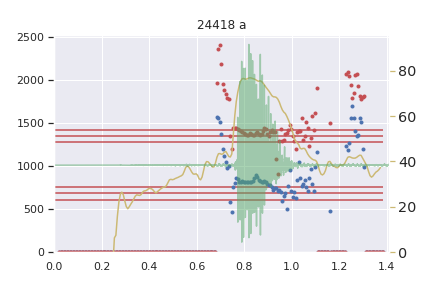
\includegraphics[width=\textwidth]{imagenes/04_02_a.png}
\end{figure}

\begin{figure}[H]
\caption{Formantes de vocal E}
\label{img:formantes_e}
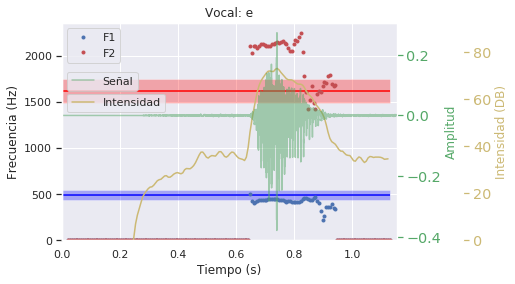
\includegraphics[width=\textwidth]{imagenes/04_02_e.png}
\end{figure}

% Esto debería estar arriba.
% En ambas figuras se muestra en verde la onda, en azul el formante 1 en rojo el formante dos, en amarillo la intensidad cuyo valor se encuentra en el eje derecho y en rojo y azul claro los rangos esperados siendo la línea centra el formante observado promedio y las lineas adyacentes los valores de sumar y restar la desviación estándar.

En la figura \ref{img:formantes_a} se observa que F2 representado por los puntos rojos está en los rangos esperados y que el F1 está cerca de los rangos esperados. En la figura \ref{img:formantes_e} se aprecia sobre la gráfica del a señal, que hay ruido de fondo, pues en los segmentos iniciales y los valores de amplitud se alejan del cero. Para esta grabación F1 se encuentra en los rangos de aceptación, pero F2 se aleja significativamente.

